\chapter{Studie}\label{Studie}
Um das System in der Praxis zu testen, musste im Anschluss eine Nutzerstudie durchgeführt werden.
Dies beinhaltete die Planung und Durchführung der Studie, sowie die Auswertung der Ergebnisse.
Es mussten die Rahmenbedingungen der Studie geplant und Testpersonen angeworben werden, die darauf in einem Interview Fragen beantworten und einen standardisierten Fragebogen zur allgemeinen Benutzung ausfüllen mussten.

\section{Entwurf}\label{Entwurf}
Nachdem die Umsetzung des Bauhausboards Systems abgeschlossen war, galt es einen Test mit Mitarbeitern der Medienfakultät der BUW durchzuführen.
\\
Dafür wurde am internen Rechenzentrum der Uni ein Linux Server mit 2,53GHz Intel Xeon Dualcore, 2GB RAM und Ubuntu Version 14.04 aufgesetzt.
Auf dem Server liefen Node.js, damit Bauhausboards ausgeführt werden konnte und Postfix\footurl{http://www.postfix.org}{10.12.2015} als Mailserver.
Dieser Mailserver konnte nur Emails an Adressen innerhalb des Universitätsnetzes verschicken, was für die Studie jedoch kein Problem darstellte.
\\
Als Displays wurden neue Tablets angeschafft, die mehr Leistung besaßen, als das Tablet aus der Vorstudie.
Es handelte sich dabei um vier Blaupunkt Discovery 1000c mit 10,1 Zoll Display, 1,33GHz AllWinner A33 Quadcore, 1GB RAM und Android 5. Mit vier Tablets konnten für die Studie vier Räume mit Displays ausgestattet werden.
\\
Damit die Benutzer, wie in der Vorstudie, nicht mit den vorinstallierten Applikationen der Tablets interagieren konnten, musste auch auf den neuen Tablets eine Kiosk-Applikation\footurl{http://www.android-kiosk.com}{10.12.2015} installiert werden.
\\
Zusätzlich zum Kiosk wurde eine Tasker-App\footurl{http://tasker.dinglisch.net}{10.12.2015} installiert.
Damit konnte man Aufgaben nach bestimmten Systemereignissen ausführen lassen.
Es wurde Task erstellt, der beim Start des Android-Systems automatisch die Kiosk-App startete, falls das System neu bootete.
\\
Als Diebstahlsicherung konnte man auf den Tablets Google Locate aktivieren.
Es diente zur Ortung der Geräte, falls diese gestohlen worden wären.
\\
\\
Um die Displays aufhängen zu können, musste eine geeignete Befestigungsmöglichkeit gefunden werden.
Jedoch sollten keine neuen Löcher zur Aufhängung an den Wänden neben den Büros entstehen.
Deswegen mussten die Displays erneut mit Hilfe der bereits aufgehängten Türschilder befestigt werden.
Da bei dieser Studie die Tablets nicht, wie in der Vorstudie, durch Löcher in der Tablet-Rückwand angebracht werden konnten, musste die Befestigung anders konstruiert werden.
Zu diesem Zweck wurden 3D gedruckte Eckstücke \abb{img:3DEckstueck}, mit denen die Tablets befestigt werden konnten, auf eine Plexiglasplatte geschraubt \abb{img:fertigeBoardaufhaengung}.
Diese Aufhängung nutzte die Bohrlöcher für die bereits vorhandenen Türschilder, wodurch keinerlei Eingriff in die Bausubstanz entstand.
% \\\todotext{Bild von den Eckstücken und von der fertigen Aufhängung}\\
\begin{figure}%[h!]
  \centering
    \subfigure[3D gedrucktes Eckstück]{
      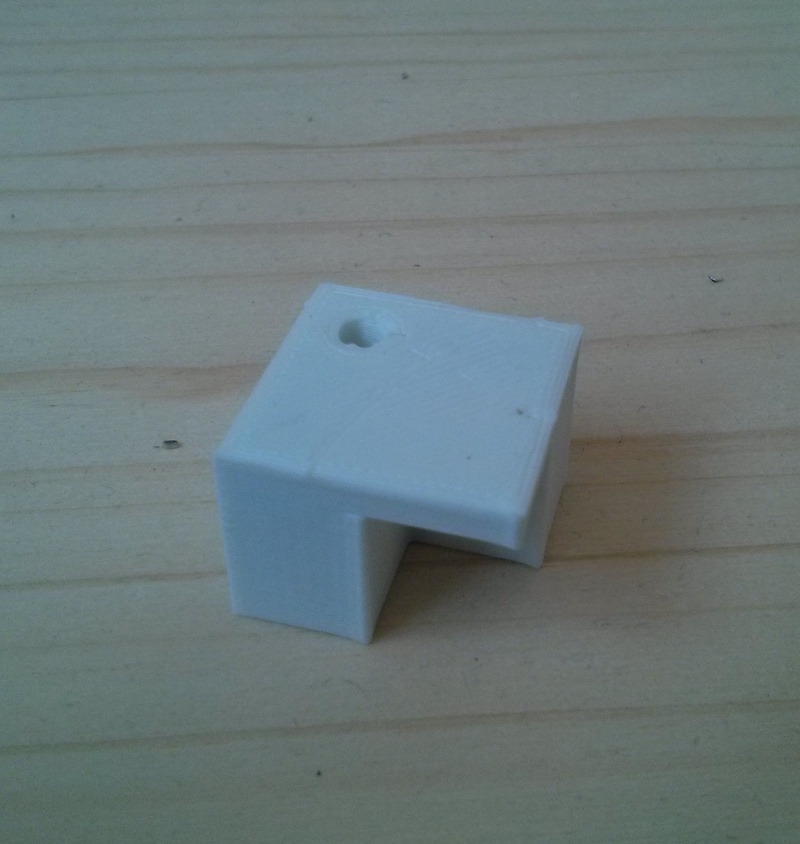
\includegraphics[width=0.327\textwidth]{./img/3DEcke.png}
      \label{img:3DEckstueck}
    }
    \subfigure[fertige Boardaufhängung]{
      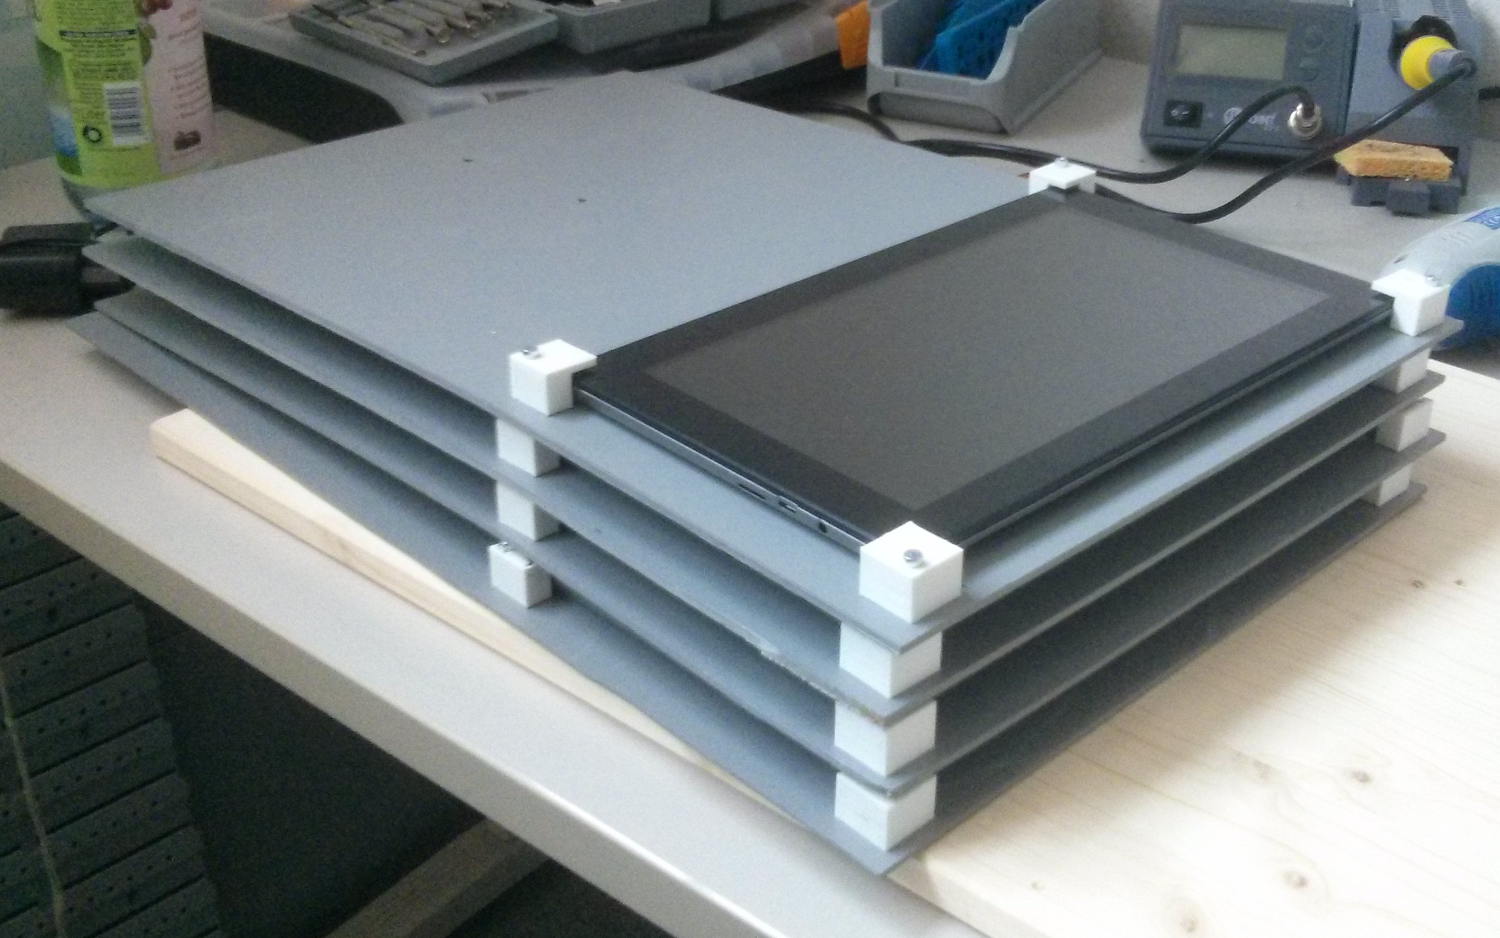
\includegraphics[width=0.55\textwidth]{./img/fertigeAufhaengung.png}
      \label{img:fertigeBoardaufhaengung}
    }
  \caption{Ergebnis der Vorarbeit}
  \label{img:Vorarbeit}
\end{figure}
\\
Damit sich die Testnutzer mit der grundlegenden Funktion von Bauhausboards vertraut machen konnten, habe ich ein Benutzerhandbuch erstellt, welches sich im Anhang befindet.
% \\\todotext{in den Anhang}.

% Nachdem Umsetzung abgeschlossen war: Test mit echten Nutzern
% Server mit NodeJS und Postfix aufgesetzt
% - Programm auf Server in Uni eingerichtet -> Spezifikationen? oder wurde das schon vorher angegeben?
% - Mailserver installiert, damit Server mails verschicken konnte (nur uni-intern)
% 4 Tablets angeschafft (Durch 4 Tablets -> 4 Räume zum Testen möglich)
%- Blaupunkt Discovery 1000c
%   * 10,1"
%   * CPU: Quadcore @ 1,33GHz
%   * Android 5.1
%   * 1GB RAM
%   * 1024x600 Auflösung (~17:10)
% Alle Tablets mit Kiosk-Mode Browser bestückt
%- Kiosk Mode Browser App auf Tablets um beenden der Bauhausboards App zu verhindern
%- Tasker zum automatischen start des kiosk modes nach systemstart - falls schlaue leute denken, sie können damit den kiosk browser umschiffen
%- Google Locate um Position des Tablets zu bestimmen, im falle eines Diebstahls
%- Rahmen: 4 Tablets -> 4 Räume
%- Wandbefestigung
%  * 3D gedruckte Eckstücke mit Loch um Tablets zu halten + zu sichern
%  * Holz/Blech Rückwand >> plexiglas
%  * Nutzung des vorhandenen Türschildes
%  * Fotos und 3D Model
%- Nutzer Tutorial zur Nutzung des Tools entworfen




\section{Durchführung}\label{Durchführung}
Da nur vier Räume mit Tablets ausgestattet werden konnten, war es nötig, mit den vorhandenen Mitteln möglichst viele Testnutzer organisieren zu können.
Mir war es möglich, einige Mitarbeiter der Professur für Systeme der virtuellen Realität (VR) und der Professur für grafische Datenverarbeitung (CG) zur Teilnahme an meiner Studie zu gewinnen.
\\
Im Fachbereich der virtuellen Realität gab es drei Büroräume.
Zwei davon mit jeweils drei und einer mit zwei Mitarbeitern.
An der Professur für grafische Datenverarbeitung gab es zwei Mitarbeiter, die sich einen Raum teilten.
Diese Räume befanden sich alle im selben Gang der Fakultät.
\\
Da ein Mitarbeiter der VR Professur durch seine Forschungsarbeit nicht in seinem Büro sein konnte, nahm er nicht an der Studie teil.
\\
Somit konnten insgesamt 9 Doktoranden und Post-Doktoranden als Testnutzer gewonnen werden.
\begin{figure}[h!]
  \centering
  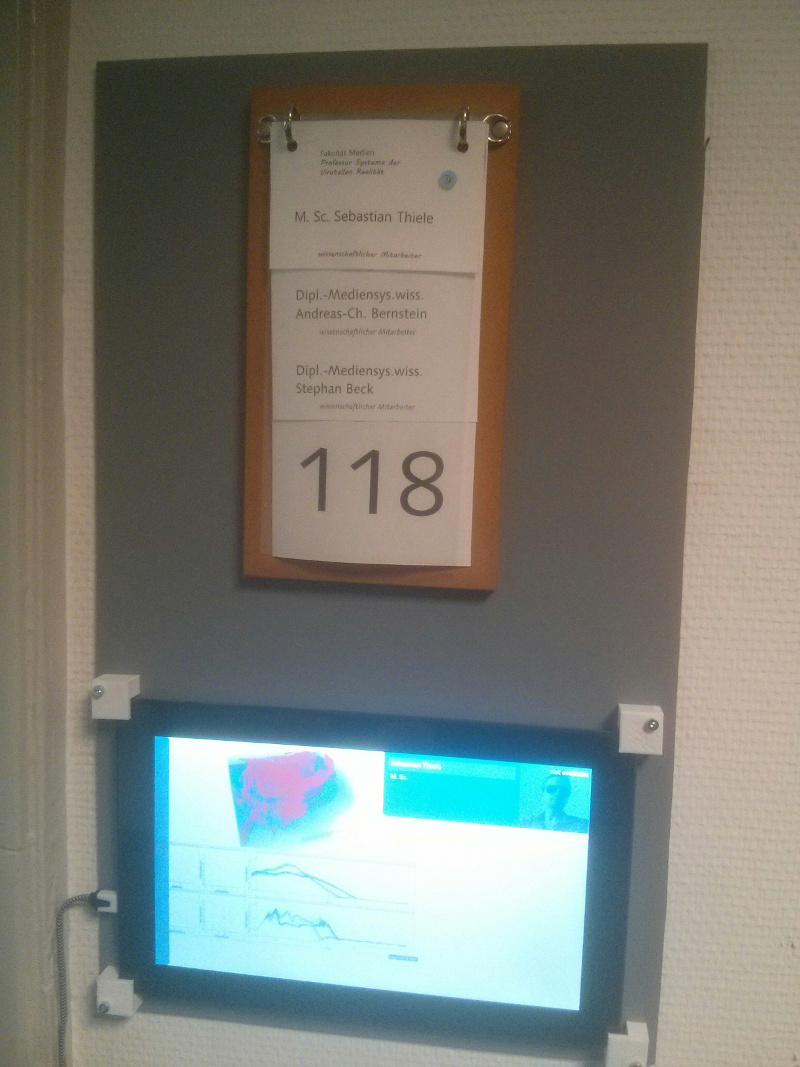
\includegraphics[width=0.4\textwidth]{./img/StudieAufgehaengtesBoard.jpg}
  \caption{Aufgehängtes Board}
  \label{img:StudieAufgehaengesBoard}
\end{figure}
\\
Bevor die Studie beginnen konnte, mussten die Boards angebracht werden \abb{img:StudieAufgehaengesBoard}.
Außerdem musste es eine gute WLAN Verbindung für sie geben, was durch zwei WLAN-Access-Points im Gang gewährleistet wurde.
% \\\todotext{Grundriss des Gangs mit Tablets + Accesspoint}\\
Nachdem die Tablets angebracht waren, wurde für jeden Benutzer ein Account erstellt, die Boards eingerichtet und die Nutzer kurz eingewiesen.
\\
Die Dauer der Studie beschränkte sich leider nur auf zwei Wochen.
Es sollte mindestens ein Wochenende eingeplant sein, weil sich das Benutzerverhalten nach diesen zwei freien Tagen ändern konnte.
\\
Während der Studie kam es gelegentlich dazu, dass einige Testnutzern Fragen zu bestimmten Funktionen hatten, welche direkt geklärt wurden.
Das System wurde gut genutzt und einige Gäste hinterließen den Testern Nachrichten.



\section{Auswertung}\label{Auswertung}
Nach Abschluss der Studie wurden alle Teilnehmer interviewt.
Um diese Interviews zu strukturieren, erstellte ich im Vorfeld einen Fragenkatalog, welcher ebenfalls im Anhang zu finden ist.
Zudem sollten die Testnutzer einen standardisierten Fragebogen zur allgemeinen Auswertung ausfüllen.
\subsection{Interview}\label{Interviews}
Der Fragenkatalog der Interviews zielte darauf ab, die Erfahrungen und Anregungen sowie das Verhalten der Nutzer im Bezug auf bestimmte Funktionen des Bauhausboards Systems herauszufinden.
\\
Zur besseren Auswertung wurden die Gespräche aufgezeichnet, wodurch ungefähr 5 Stunden und 30 Minuten an Gesprächsmitschnitten entstanden. 
\\
Die Fragen wurden in unterschiedliche Kategorien geteilt.
Es ging darum herauszufinden, wie es für die Testnutzer war, Nachrichten zu empfangen und ob sie selber Nachrichten geschrieben haben.
Außerdem wurde die Benutzung des Status- und Inhalts-System evaluiert und es musste herausgefunden werden, wie die Testnutzer die Benutzung des Editors fanden.
Zum Schluss wurden sie danach gefragt, was sie von den allgemeinen Boardfunktionen hielten und was sie für zusätzliche Anmerkungen haben.
\subsubsection{Nachrichten empfangen}\label{Nachrichten Empfangen}
% \todotext{ein bild einer Nachricht}\\
\begin{figure}[h!]
  \centering
  \frame{
\includegraphics[width=0.4\textwidth]{./img/StudieMessageExample.png}}
  \caption{Ein Beispiel einer Spaß-Nachricht}
  \label{img:StudieExampleMessage}
\end{figure}
Als erstes ging ich mit den Testnutzern deren empfangenen Nachrichten durch.
Ich fragte sie, um was es in diesen Nachrichten ging.
Es galt herauszufinden, wofür die Besucher die Nachrichtenfunktion genutzt haben.
\\
Dies waren größtenteils Spaßnachrichten \abb{img:StudieExampleMessage} oder hatten keinen speziellen Bezug. Ein Testnutzer bezeichnete seine erhaltenen Nachrichten als ``temporäres Graffiti''.
Teilweise gab es auch Nachrichten mit direktem Bezug.
Ein paar Nutzer wurden durch die Nachricht gefragt, ob sie mit dem Autor essen gehen wollten oder wurden auf ihren angezeigten Inhalt angesprochen.
Außerdem wurde ein Nutzer gefragt, ob er zur Zeit in der Uni anzutreffen war.
\\
Ein weiterer Bestandteil der Befragung war, wie die Autoren der Nachrichten identifiziert werden konnten.
Alle Nachrichten, die während der Studie erstellt wurden, hatten keine Autorenkennzeichnung.
Das wurde von den meisten Testnutzern als größte Schwäche bemängelt, da sie bei bestimmten Nachrichten nur raten konnten, wer sie erstellt hatte.
\\
Interessant war es zu wissen, wie die Testnutzer, alternativ zu Bauhausboards, für Gäste erreichbar waren.
Der Großteil meinte darauf, dass sie üblicherweise per Mail erreichbar waren.
Andere meinten, Besucher könnten sie per Post-It-Zetteln oder Klopfen an ihrer Tür erreichen.
\\
Für die Kommunikation untereinander gaben einige an, Telefon, SMS oder Instant-Messenger zu nutzen.
\\
Auf die Frage, wie schnell die Testnutzer ihre Nachrichten gelesen haben, meinten alle (bis auf einen), dass sie direkt die Mail erhalten und auf den eingebetteten Link geklickt haben.
Die Funktion des direkten Nachrichtenaufrufs per Link in der Email wurde von allen Testnutzern als sehr gut empfunden, da sie sich somit nicht extra im System anmelden mussten.
\\
Ich fragte die Nutzer, ob es für sie in irgend einer Form anders war, über das Board eine Nachricht zu erhalten.
Da mit dem System Zeichnungen verschickt werden konnten meinte ein Testnutzer, dass es eine persönliche Note verschafft: ``Die Zeichnungen machen es anders''.
Die Anderen sahen es als eine normale Email-Nachricht, was demnach gut war.
Es wurde besonders gut aufgenommen, dass die Tester von den Besuchern über das System angesprochen werden konnten, wenn sie sich derzeit nicht im Büro aufhielten und die Besucher dafür nicht extra ein eigenes Gerät benötigten.
\\
Zur Verbesserung des Nachrichtensystems meinten einige, dass es vereinfacht werden müsste, da sie es als zu kompliziert erachteten.
Es sollten weniger Klicks notwendig sein, bis eine Nachricht abgeschickt werden könne und weniger Untermenüs enthalten.
Außerdem meinten sie, dass die Funktion eine Nachricht an mehrere Personen gleichzeitig erstellen zu können nicht gebraucht wird.

% Nachrichten empfangen
%  - mit den Nutzern die empfangenen Nachrichten durchgegangen um Herauszufinden, wofür die Gäste die Funktion genutzt haben
%  - Größtenteils keine ernst gemeinten Nachrichten (Spaßnachrichten, ``temporäres Grafitty'')
%  - ab und an Fragen, ob man zusammen Mittag essen gehen will oder ob Nutzer zugegen ist

%  - es war in keiner Nachricht ersichtlich, wer deren Autor war
%  - wurde von den Meisten Testnutzern bemängelt, dass sie den Autor nicht identifizieren konnten (sie konnten nur ab und an vermuten, wer es war)

%  - Nutzer wurden gefragt, wie man ihnen sonst eine Nachricht hinterlassen konnten
%  - die meisten meinten: per mail
%  - aber auch: postIt, tel, klopfen, sms(dafür müssen aber kontaktdaten da sein), usw

%  - Nutzer gefragt, ob es für sie anders war, über das Board eine Nachricht zu erhalten
%  - war praktisch, ``Die Zeichnung macht es anders'' (also positiv, dass Zeichnungen drin waren) es schafft eine persönliche Note, aber für manche war es nicht anders als eine normale mail(und demnach gut)

% - Alle haben dadurch, da sie per mail benachrichtigt wurden, es direkt gelesen, da sie auch direkt auf den link in der mail klicken konnten und sich deswegen nicht extra anmelden mussten

% - einige Nutzer fanden es gut, dass man ihnen eine Nachricht hinterlassen konnten, wenn sie grade nicht im Büro waren
% - als größtes Manko empfanden die Testnutzer, dass sie nicht sehen konnten, wer die Nachricht geschrieben hat
% - andere fanden es zu umständlich, einen einfachen text einzugeben, da die Touchauflösung des Tablets zu gering war
% - außerdem wurde es gut aufgenommen, dass man für die KOmmunikation mit den Besitzern nicht extra ein eigenes Gerät brauchte, da die Boards vor den Büros hingen

% - Verbesserungsvorschläge: autorkennzeichnung, voicemail, videomail, Vordefinierte Nachrichtenkategorien(dem Anliegen entsprechend), Vereinfachung durch weniger untermenüs



% FAZIT
% -> option für autorenmarking einbauen
% ->
% -> KOmmunikation per mail, sms, tel setzt wissen der kontaktdaten vorraus
% -> Kommunikation per postIt: da kann man Zettel klauen
%%%%%%%%%%%%%%%%%%%%%%%%%%%%%%%%%%%%%%%%%%%%%%%%%%%%%%%%%%%%%%%%%%%%%%%%%%%%%%%%
\subsubsection{Nachrichten schreiben}\label{Nachrichten schreiben}
Ich fragte die Testnutzer, ob sie in der Laufzeit der Studie einem anderen Nutzer eine Nachricht hinterlassen haben.
Die meisten meinten jedoch, dass sie nur über die Besitzerrolle das System nutzten, weil sie entweder keine Zeit hatten jemanden eine Nachricht zu schreiben oder persönlich mit diesen Personen redeten.
Da sich die Testnutzer untereinander gut kannten, war es für sie einfacher, miteinander zu reden anstatt über das Board eine Nachricht zu schreiben.
Einem der Nutzer war der Prozess, eine Nachricht zu erstellen, zu aufwändig und hat deswegen keine Nachrichten geschrieben.
% selber Nachrichten schreiben
% - Auf die Frage, ob die Testnutzer einem anderen Besitzer eine Nachricht auf ihr Board hinterlassen haben, meinten die meisten, dass sie selber nur die Besitzerrolle wahrgenommen hatten und keinem eine Nachricht hinterlassen haben
% - das hatte den Grund, da sich die meisten Tester persönlich sehr gut kannten und die meiste Kommunikation mündlich durchführten
% - Einem Nutzer war der ganze Nachrichtenprozess zu viel Aufwand (und es war ihm zu versteckt)
% - ein paar Testnutzer nutzen es, um einen anderen Nutzer zu fragen, ob er mit zum Mittagessen mitkommen wollte
%%%%%%%%%%%%%%%%%%%%%%%%%%%%%%%%%%%%%%%%%%%%%%%%%%%%%%%%%%%%%%%%%%%%%%%%%%%%%%%%
\subsubsection{Nutzerinhalt}\label{Nutzerinhalt}
% \todotext{ein Bild von einem guten Content}\\
Am wichtigsten war es, herauszufinden, was die Testnutzer während der Studie für Inhalte erzeugten und wie für die Benutzung dieses Features war.
Hauptsächlich wurde es dazu genutzt, um Spaß-Informationen zu präsentieren.
Dazu wurden meist Bilder und Gifs hochgeladen.
Von einigen Nutzern wurde dieses Feature auch genutzt, um die aktuelle Arbeit zu beschreiben \abb{img:StudieExampleContent}.
Einer meinte, er nutze es gern ``um von außen einen schnellen Eindruck zu gewähren, was er macht''.
\begin{figure}[h!]
  \centering
  \frame{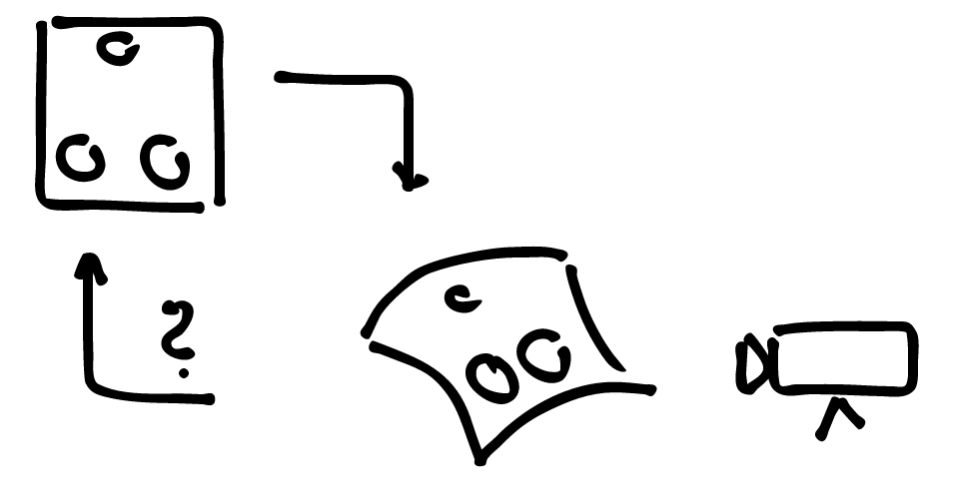
\includegraphics[width=0.7\textwidth]{./img/StudieContentExample.png}}
  \caption{Ein Beispiel eines Nutzerinhalts zur aktuellen Arbeit}
  \label{img:StudieExampleContent}
\end{figure}
\\
Einige Tester nutzten diese Funktion zum Anzeigen ihres Status, obwohl es dafür ein eigenes Feature gab.
\\
Ansonsten wurde die Hintergrundschicht von einigen zur Anzeige von Webseiten, wie die Seiten der jeweiligen Professur, genutzt.
Ein Nutzer meinte, dass der Editor zum Erzeugen von Inhalt vollkommen ausreichen würde und die Hintergrundschicht maximal als Poweruser\footnote{ein Poweruser ist ein Nutzer, der deutlich mehr Kenntnisse über das System hat, als normale Nutzer}-Funktion angeboten werden sollte.
\\
Leider nutzte keiner der Tester die Twitterfunktion.
Das lag daran, da alle Tester, bis auf einen, keinen Twitteraccount besaßen.
Dieser wollte jedoch nicht seine privaten Twittermeldungen in der Universität präsentieren.
\\
\\
Einige Tester fanden den Ansatz der Informationsdarbietung interessant, da es eine neue Technologie war und man damit sogar bewegten Inhalt erstellen konnte.
\\
Bedauerlicherweise gab es auch Nutzer, die das Feature gar nicht nutzten.
Diese meinten jedoch, dass sie keine Zeit hatten, einen Inhalt zu erstellen oder ihnen einfach nichts eingefallen ist.
\\
% Auf die Frage, ob es Besucher gab, die auf den Inhalt der Tester eingegangen sind 
Es war zudem sehr erfreulich, dass es Besucher gab, die auf den Inhalt einiger Testern eingegangen sind und diese explizit darauf angesprochen haben.
Dadurch wurde sogar über das System eine Gesprächsgrundlage geschaffen.
\\
\\
Die Inhaltsfunktion als solche wurde von den meisten positiv aufgenommen, da sie einen persönlichen Aspekt bot: ``Sehr gut war die Möglichkeit, selber Kreativ zu werden''.
Zudem wurde es begrüßt, dass über das Board Informationen, Bilder und animierte Gifs präsentiert werden konnten.
\\
Einige waren jedoch der Meinung, dass das System zu kompliziert sei und es zu viele Funktionen bot.
Einem Nutzer waren es zu viele Schritte nötig, bis er seinen Inhalt ändern konnte.
% Content ändern
% - der Content wurde hauptsächlich für spaß benutzt, es wurden Bilder und gifs hochgeladen und präsentiert. Aber es wurde auch zum Teil zur präsentation von fachlichem Inhalt verwendet ``um von außen einen schnelleren Eindruck zu gewähren, was ich mache''
% - andere Nutzen diese Funktion wie schon gesagt zur ANzeige ihres Status

% - entweder wurde der Editorlayer oder aber der Backgroundlayer zur Anzeige von Bildern/Gifs genutzt weil es war für die NUtzer nicht offensichtlich, wie man im Editorlayer bilder hochlädt --> einbau eines buttons dafür
% - genutzt für Webseiten (Nachrichten oder Seite der Professur)
% - Backgroundlayer wurde größtenteils positiv aufgenommen, wäre aber besser als poweruserfunktion
% - ein Nutzer meinte: Nutzer sollten selber über Background-Interaktivität entscheiden können

% - alle Nutzer haben nicht das twitterfeature genutzt, da fast alle keinen twitteraccount hatten
% - der eine Nutzer, der einen acc hatte, würde das feature nicht nutzen, da er privaten inhalt sonst präsentieren müsste

% - übliche änderungszeit war zur Mittagszeit in der pause
% - leider ist benutzung mit der zeit eingeschlafen (nur am anfang der studie, danach weniger genutzt)

% - NUtzer fanden es interessant, da technologie neu war, man bewegten Inhalt präsentieren konnte oder einfach nur aus spaß
% - die nutzer, die es nicht benutzten hatten entweder keine Zeit einen content zu erstellen oder ihnen ist nichts eingefallen

% - schön war es, dass es ab und an auch gäste gab, die auf den content von besitzern eingegangen sind und ein gespräch deswegen entstanden ist

% - von den meisten wurde es positiv aufgenommen: der persönliche Aspekt ``Sehr gut war die Möglichkeit selber Kreativ zu werden''
% - auch gut war es, dass man damit INformationen präsentieren konnte
% - am besten fanden die TEster, dass man damit gifs anzeigen konnte

% - einige Benutzer fanden wieder die bedienung zu kompliziert und, dass es zu viele features gab, dass man es auch hätte vereinfachen können
% - zu viele schritte, bis content geändert wurde --> weniger klicks desto besser

% - es wäre wahrscheinlich ernster benutzt worden, wenn es ganz offiziell da hängen würde oder es kommuniziert worden wäre, für welchen Content es vorrangig genutzt werden sollte
%%%%%%%%%%%%%%%%%%%%%%%%%%%%%%%%%%%%%%%%%%%%%%%%%%%%%%%%%%%%%%%%%%%%%%%%%%%%%%%%
\subsubsection{Status}\label{Status}
Die meisten Tester haben diese Funktion gelegentlich genutzt.
Einige haben ihren Status jedoch lieber mit der Inhaltsfunktion angegeben.
% Alle Tester haben ihren Status vom Desktop-PC geändert
Nur ein Nutzer gab seinen Status beim Verlassen des Raumes am Board an, die anderen taten dies an ihrem PC.
\\
Als Statustexte wurde zum Beispiel angegeben, ob man derzeit beschäftigt war: ``busy'' oder wo man zu finden ist: ``im DBL zu finden''.
\\
Einige Nutzer waren der Meinung, dass es zu kompliziert ist, einen Status zu setzen.
Es waren ihnen zu viele Klicks notwendig und das Interface zu schwer zu bedienen.
\\
Von einigen Testnutzern wurde es gut aufgenommen, dass es diese Funktion gab und dass sie damit angeben konnten, wo sie sich befanden oder nicht gestört werden wollten.
Zudem wussten Gäste dadurch, wann ein bestimmter Nutzer wieder anzutreffen war und mussten sich nicht bei dessen Kollegen nach ihm erkundigen.
\\
Auf die Frage, ob die Nutzer das Feature häufiger verwenden würden, wenn es vordefinierte Status geben würde, antworteten die meisten mit ja.
Die anderen meinten, dass sie es nicht für nötig hielten, ihren aktuellen Status anzugeben, da sie eh die meiste Zeit im Büro waren.
Sie sahen es als impliziten Status an, wenn sie entweder nicht da waren oder ihre Tür geschlossen war: ``Wenn die Tür zu ist, bin ich nicht da''.
\\
Die Gespräche ergaben, dass die Funktion zur Abwesend-Markierung fast nicht benutzt wurde und deswegen nicht weiter gebraucht wird.
\\
Einige Tester meinten, dass der Status im Header zu unoffensichtlich ist und daher besser gekennzeichnet werden sollte.

% Statusfunktion
% - die meisten Testnutzer haben die Funktion direkt genutzt oder aber sich ihren Status auf ihre Pinnwand geschrieben
% - davon haben alle Nutzer bis auf einen die Funktion vom PC aus genutzt, der andere wollte es am Board ändern, war aber der meinung, dass es für ihn zu kompliziert war, den status zu ändern (der meinung waren auch einige andere Testnutzer)
% - übliche Statustexte waren: ``busy'' oder ``im DBL zu finden'' oder im Meeting oder ganz einfach N/A
% - wie gesagt einige fanden das system zu kompliziert, vorallem das Interface (es bot zu viel auf einmal und war zu schwer zu erreichen)
% - andere wiederum fanden es gut, dass es dieses feature gab und man gesondert seinen aktuellen status kennzeichnen konnte
% - nützlich für gäste, um zu wissen, wann der Besitzer wieder da ist
% - Kollegen von Testnutzern mussten nicht wegen dessen status behelligt werden 
% - die meisten Nutzer haben den Status vor dem Verlassen des Büros geändert, wenn sie essen gegangen sind oder ins Meeting
% - auf die Frage ob Vordefinierte Status sie eher dazu animieren würden, das Feature zu nutzen meinte die Mehrzahl, dass es das würde

% - Die Auswertung ergab, dass die N/A Funktion zum Ausgrauen des Nutzerbildes nicht gebraucht wird

% - viele meinten, dass der Status zu unoffensichtlich ist und besser gekennzeichnet werden müsste oder komplett heraus genommen werden sollte, da man das auch alles über den COntent machen könnte
% - Ein Nutzer meinte, er würde seinen Status nur von unterwegs ändern, wenn er dem system eine mail mit dem statustext schicken könnte oder es per app machen könnte
% - Die Funktion sollte komplett vom Board genommen werden und nur für die Desktop-Version zugägnlich sein

% - der grund warum einige das Feature nicht genutzt haben war, dass ``sie eh die ganze Zeit da waren und es deswegen nicht brauchten'' oder es nicht für nötig hielten, da eine geschlossene Tür schon statusindikator genug ist ``Wenn die Tür zu ist, bin ich nicht da''
%%%%%%%%%%%%%%%%%%%%%%%%%%%%%%%%%%%%%%%%%%%%%%%%%%%%%%%%%%%%%%%%%%%%%%%%%%%%%%%%
\subsubsection{Editor}\label{Editor}
Fast alle Tester haben den Editor genutzt, um sich Inhalt zu erzeugen.
Es wurden eigene Arbeiten skizziert, Texte geschrieben oder einfach nur Spaßzeichnungen erstellt.
\\
Da die Icons nicht wie in üblichen Editoren waren, konnten sie nicht alle eindeutig identifiziert werden, was von den meisten Testern bemängelt wurde.
Sie hätten es besser gefunden, wenn die Gestaltung der Icons sich nach den üblichen Standards richten würde.
\\
Da manchen Benutzern anfangs nicht klar war, dass sie Bilder und Gifs per Drag-and-Drop hochladen konnten, nutzten sie dafür nur die Hintergrundschicht.
Die Mehrzahl der Nutzer meinte deswegen, dass eine eigene Schaltfläche, um Bilder hochladen zu können, angebrachter wäre.
\\
Einigen Testern war es beim Zeichnen nicht klar, welches Werkzeug sie zur Zeit ausgewählt hatten und wünschten sich eine bessere Kennzeichnung.
\\
Es wurde sich positiv über die Benutzung des Editors geäußert.
Einige Tester meinten, dass der Editor allein schon vollkommen als einzige Bauhausboardfunktion ausreichen würde.


% Editor Benutzung
% - fast alle (außer 2) haben den Editor benutzt
% - sie haben es dafür benutzt um bspw eigene Arbeit zu skizzieren, texte zu zeichnen oder einfach nur spaßzeichnungen zu machen
% - die anderen meinten die benutzung wäre zu versteckt im backend
% - da die icons nicht wie in den üblichen editoren waren, waren sie nicht eindeutig(color=underline,selector wie rectangleZeichnen,undo-redo->geschwungene pfeile)
% - einigen war nicht von anfang an bewusst, dass sie bilder und gifs per drag and drop einbinden können (sie benutzten dafür die hintergrundlayer) -> musste ihnen erst gezeigt werden   ---> lieber Hinweis auf Funktion machen + extra upload button
% - es war schlecht, dass es keine autoskallierung für bilder und keine vordefinierten formen gab
% - außerdem wurde es bemängelt, dass das ausgewählte werkeug zu wenig hervorgehoben wurde

% - positiv war, dass er recht intuitiv zu benutzen war, dass er postIt ähnlich war

% - ``Es war für den Rahmen in dem es lief ausreichend''
% - ein Nutzer meinte, dass das schon allein als Boardfeature reichen würde
% - ausmalfeature wäre noch gewünscht
% - wekzeuge sollten dauerhaft angezeigt werden
%%%%%%%%%%%%%%%%%%%%%%%%%%%%%%%%%%%%%%%%%%%%%%%%%%%%%%%%%%%%%%%%%%%%%%%%%%%%%%%%
\subsubsection{Boardfunktionen}\label{Boardfunktionen}
Für einige Testnutzer war es nicht ersichtlich, wo sie sich im Backend befanden und ob sie noch angemeldet sind.
Deswegen war es der Wunsch von mehreren Benutzern, das Frontend auch vom Benutzer-Backend zu trennen und auf den Displays nur das Frontend anzubieten.
\\
Zudem sollte der durchschnittliche Klickaufwand reduziert werden, damit sich Funktionen schneller durchführen lassen.
\\
Als sie nach den Authentisierungsmethoden gefragt wurden, meinten die meisten, dass zwei Authentisierungen übertrieben sind.
Wenn das Frontend vom Backend getrennt wäre, bräuchte man nur ein Passwort am Backend.
Einer der Nutzer war sogar der Meinung, die Authentisierung komplett weg zu lassen ``auch wenn es Vandalismus Tür und Tor öffnet''.
\\
Außerdem waren einige Tester nicht mit dem zeitlichen Wechsel der Nutzer einverstanden.
Sie hätten es lieber gehabt, wenn alle Nutzer parallel angezeigt werden, wodurch alle Benutzer und deren Status auf einen Blick sichtbar wären.
\\
\\
Ich fragte die Testnutzer, was sie in Bauhausboards als Vorteil oder Nachteil gegenüber Post-It's, Whiteboards und Pinnwänden sehen.
Fast alle Benutzer meinten, dass sehr gut war, dynamischen Inhalt erstellen zu können und dass sie über Besuchernachrichten informiert werden.
Die Boards produzieren nicht wie Post-It's Müll und können nicht einfach entfernt werden.
Zudem wissen nur der Ersteller und der Empfänger einer Nachricht deren Inhalt.
\\
Als Nachteil wurde die Tatsache angesehen, dass die Boards kontinuierlich Energie verbrauchen und teurer als Post-It's sind.
Einer der Testnutzer war der Meinung, dass die Boards im Vergleich zu Post-It-Statusmeldungen nur periphere Aufmerksamkeit erzeugen.

% Allgemeine Boardfunktionen
% - es war für einige Tstnutzer nicht ersichtlich, wo sie sich im backend befanden, ob sie noch angemeldet sind und wer überhaupt angemeldet ist
% - deswegen sollte lieber das BAckend vom Frontend getrennt werden und vereinfachen (da jetzt zu viele klicks notwendig waren)
% - Alle Nutzer waren der Meinung, dass 2 Authentisierungen übertrieben sind
% - wenn Frontend und Backend getrennt wären, bräcuhte man nur eine Authentisierungsmethode
% - ein Nutzer war sogar der Meinung Passwortauthentisierung komplett weg zu lassen ``auch wenn es Vandalismus Tür und Tor öffnet''

% Frage, was sie als Vor- und Nachteile gegenüber PostIts, Whiteboards und Pinnwänden sehen
% positiv:
% - digitaler/dynamischer content
% - produziert keinen müll
% - die Besitzer werden direkt über Nachrichten informiert(per mail)
% - privacy(nur empfänger kann nachricht lesen)
% - keiner kann Nachricht löschen - postIt/whiteboardnachrichten aber entfernbar
% - Erstellung von Content per Remote
% - Kontaktaufnahme, selbst wenn Kontaktdaten unbekannt oder man kein geeignetes device zur hand hat
% - macht spaß
% - daten werden archiviert

% negativ
% - kostet energie
% - teurer als postIts
% - wird nur als spielerei wahrgenommen + Statusmeldungen im endeffekt nur peripher von Gästen wahrgenommen (postIts werden ernster genommen)

% - Die Größe der Boards fanden alle angemessen und hätten nicht unbedingt größere Boards gebraucht

% - viele waren der Meinung, dass der Wechsel zwischen den Benutzern nervig war
% - sie hätten lieber gewollt, dass die Nutzer parallel angezeigt werden, sodass man dann direkt auf den Benutzer klicken könnte um ihn eine Nachricht zu schreiben
% - dadurch hat man auch eine direkte sicht darauf, wer alles im Raum arbeitet, wer davon grad nicht verfügbar ist und was so dessen Status ist
% - dafür wäre auch in Kauf genommen, dass nur 1/3 Platz für Content zu Verfügung steht


%%%%%%%%%%%%%%%%%%%%%%%%%%%%%%%%%%%%%%%%%%%%%%%%%%%%%%%%%%%%%%%%%%%%%%%%%%%%%%%%
\subsubsection{Allgemeine Anmerkungen}\label{Allgemeine Anmerkungen}
Leider war die Laufzeit der Studie nur zwei Wochen, wodurch die Testnutzer nur sehr wenig Zeit hatten, sich an die Boards zu gewöhnen und deren Funktionalität in ihren Arbeitsprozess mit einzubinden.
\\
Einige der Nutzer empfanden es als lästig, dass die Sidebar sich nach einer kurzen Zeit selbstständig schloss:
``Du sitzt am Schreibtisch, arbeitest und hast dir deine Werkzeuge hingelegt. Dann kommt ständig deine Freundin und räumt sie wieder weg.''
Deswegen sollte sie bei der Benutzung des Editors entweder dauerhaft angezeigt oder die Editorwerkzeuge ausgelagert werden.
\\
Ein Nutzer meinte, dass die Boards sehr gute Notleuchten für den Gang sind, da sie im Dunkeln ausreichend Beleuchtung boten.


% Allgemeine Anmerkungen
% - Studie war zu kurz um sich wirklich dran zu gewöhnen, weswegen die Funktionalität nicht in den Arbeitsprozess mit eingegangen ist
% - Teilweise waren die Menüpunkte nicht eindeutig bezeichnet
% - ``es war schön, dass man darüber Nachrichten empfangen konnte''
% - Für einen Testnutzer war es zu viel Aufwand, wenn man etwas auswählen musste oder durch das menü navigieren musste ``Keiner möchte ewig vor seinem Büro stehen und da rum klicken'' --> deswegen Trennung Frontend/Backend
% - Am besten wäre für zusätzliche Funktionalität eine Poweruser Einstellung
% - ein Nutzer meinte die Boards sind gute Notleuchten und dass sie gute Blickfänger sind
% - status Die Funktion sollte komplett vom Board genommen werden und nur für die Desktop-Version zugägnlich sein

% Sidebar:
% - viele fanden es nervig, dass die sidebar immer wieder zu ging
% --> lieber auf Desktop dauerhaft anzeigen
% - autoclose nervig im Editor ``Du sitzt am Schreibtisch, arbeitest und hast dir deine Werkzeuge hingelegt. Dann kommt ständig deine Freundin und räumt dein zeug weg.''

% Board:
% - Touch genauigkeit zu unpräzise
%%%%%%%%%%%%%%%%%%%%%%%%%%%%%%%%%%%%%%%%%%%%%%%%%%%%%%%%%%%%%%%%%%%%%%%%%%%%%%%%



\subsection{UEQ Fragebogen}\label{UEQ Fragebogen}
Um das System zusätzlich auszuwerten sollten die Testnutzer einen Fragebogen ausfüllen.
Das User Experience Questionaire\footurl{http://www.ueq-online.org}{10.12.2015} (UEQ) ist eine einfache und schnell durchführbare Möglichkeit, interaktive Systeme zu evaluieren.
Es beinhaltet einen Fragebogen mit 26 sorgfältig ausgewählten Fragen zu 6 Klassen: Attraktivität, Durchschaubarkeit, Effizienz, Steuerbarkeit, Stimulation und Originalität.
Zu jeder Frage gab es 7 Ankreuzmöglichkeiten. Sie gingen von -3 (unattraktiv) bis 3 (attraktiv).
Diese Fragen durften nicht abgeändert oder entfernt sowie keine neuen hinzugefügt werden.
\begin{figure}[h!]
  \centering
    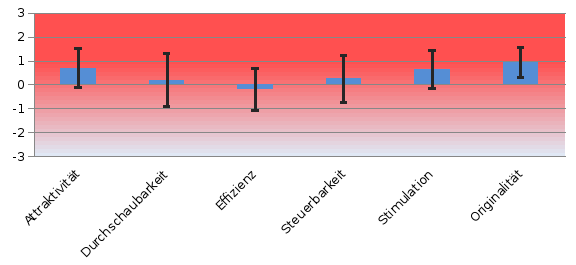
\includegraphics[width=0.9\textwidth]{./img/UEQ_Scales.png}
  \caption{UEQ - Klassen}
  \label{img:UEQScales}
\end{figure}
\\
\\
In Abb. \ref{img:UEQScales} kann man erkennen, dass die Testnutzer das System vorwiegend als Attraktiv, Stimulierend und Originell empfanden.
\\
Da Bauhausbaords ein neues System für die Testnutzer war, ist die Attraktivität annähernd bei 1 und daher positiv.
\\
Viele Nutzer meinten, dass es im Gang eine höhere Aufmerksamkeit erzeugte. Zum einen, da die Tablets von selbst leuchten und zum anderen, da sie animierte Gifs anzeigen können. Deswegen ist das Ergebnis in der Klasse Stimulation ungefähr 1 ebenfalls positiv.
\\
Die Idee, digitale Türschilder zu benutzen schienen die Tester als Originell zu empfinden, da es im Diagramm den höchsten Durchschnittswert erreichte.
\\
Die Werte für die Klassen Durchschaubarkeit, Effizienz und Steuerbarkeit sind annähernd neutral.
Dies liegt möglicherweise daran, da für einige Benutzer manche Funktionen zu kompliziert waren und zu viele Klicks erforderten.
Einige Funktionen waren zudem nicht auf den ersten Blick ersichtlich und die Genauigkeit des Touch-Interfaces für manche Nutzer zu ungenau.
\\
\\
Diese Werte überdecken sich in gewisser Hinsicht mit dem Ergebnis des Interviews.
% \\\todotext{hier noch mehr zu UEQ?}
% UEQ Fragebogen nach Testlauf
% was ist UEQ
% 26 Fragen zur evaluierung
% Fragen dürfen nicht separiert, da Ergebnisse sonst nichtmehr gültig



% Ergebnisse des UEQ
% - !! wirklich nur 9 Testnutzer, deswegen nur bedingt Aussagefähig
% - Angabe der Mean Results Tabelle
% - und Mean Value per Item
% --> alles durchschnittlich bis gut, außer Effizienz schlecht (Zurückzuführen auf die Touchgenauigkeit des Tablets)
